\documentclass[11pt,a4paper]{article}
\usepackage[T1]{fontenc} 
\usepackage[utf8]{inputenc}
\usepackage[english]{babel} 
\usepackage{verbatim}
\usepackage{graphicx}
\usepackage{acronym}
\usepackage{url}
\usepackage{cite}
\usepackage{amsmath}

\begin{document}

\section{Chapter 3: Implementation}
\subsection{Simulation/Emulation of gossip-based aggregation}
To evaluate the value of the gossip-based aggregation it is necessary to see it in the wild of a real network environment. Unfortunately the setup of a real network is to time and cost intensive. Hence the next best thing was chosen: A network emulation. In a network simulation the network is simplified so as to illuminate a certain set of behaviours (e.g. ns \cite{ns}). An emulation in contrast consists of all the elements of the real network only that the resources are not "real" but "virtual". While for example an emulated switch may process network traffic in the very same way as a switch in your office, it could be implemented as a linux process.

In this research the netkit emulation framework (itself a wrapper to user mode linux \cite{uml}) was chosen. Netkit \cite{netkit} creates virtual linux machines from a set of configuration files. These virtual machines are automatically connected through usermode processes called "uml\_switch". It is possible to logon to the machines via ssh and configure them just like any other linux machines. This allows great freedom to try and test software which otherwise would be hard to implement.

The initial set of configuration files were created with the tool Autonetkit \cite{autonetkit} using network graphs from the "Topology Zoo" \cite{knight_internet_2011}. The "Topology Zoo" is a collection of around two hundred fifty graphs of telecommunication networks. The graphs are open for use and give a good idea on the reality of communication networks. Simon Knight, one of the founders of the topology zoo has developed the tool Autonetkit. It takes a graph xml file (graphml) and constructs over a series of abstractions configuration files (from OSPF to DNS). For the purpose of this experiment Autonetkit was augmented so as to create for our gossip agent a file containing all neighbours of the individual nodes.

\subsection{Implementation of gossip-based aggregation daemon}
As the gossip agent in our emulated network we developed a daemon based on the pseudo code of the gossip-based aggregation algorithm (REF: section 2 or article). The programming language Python \cite{python} was chosen for this task as it's simplicity and clarity enable a rapid development. Packets between nodes were exchanged in short lived TCP conections. The daemons on the individual nodes are started from outside the emulation system and write a log and results to the host system. After a number of periods (epochs) the daemons exit.

Two threads are coexisting (see figure \ref{fig:flow_diag}). The active thread connects to randomly chosen neighbours at a predefined interval (epoch duration). The passive thread accepts connection all the time. Each thread update a state after a succesful connection. To make the state develop linearly both threads have to compete for a lock before establishing a connection. (Combining multithreading with networking led to some problems, especially when two nodes chose to actively create a connection with each other at the same time.)
\begin{figure}[h!]
    \begin{center}
        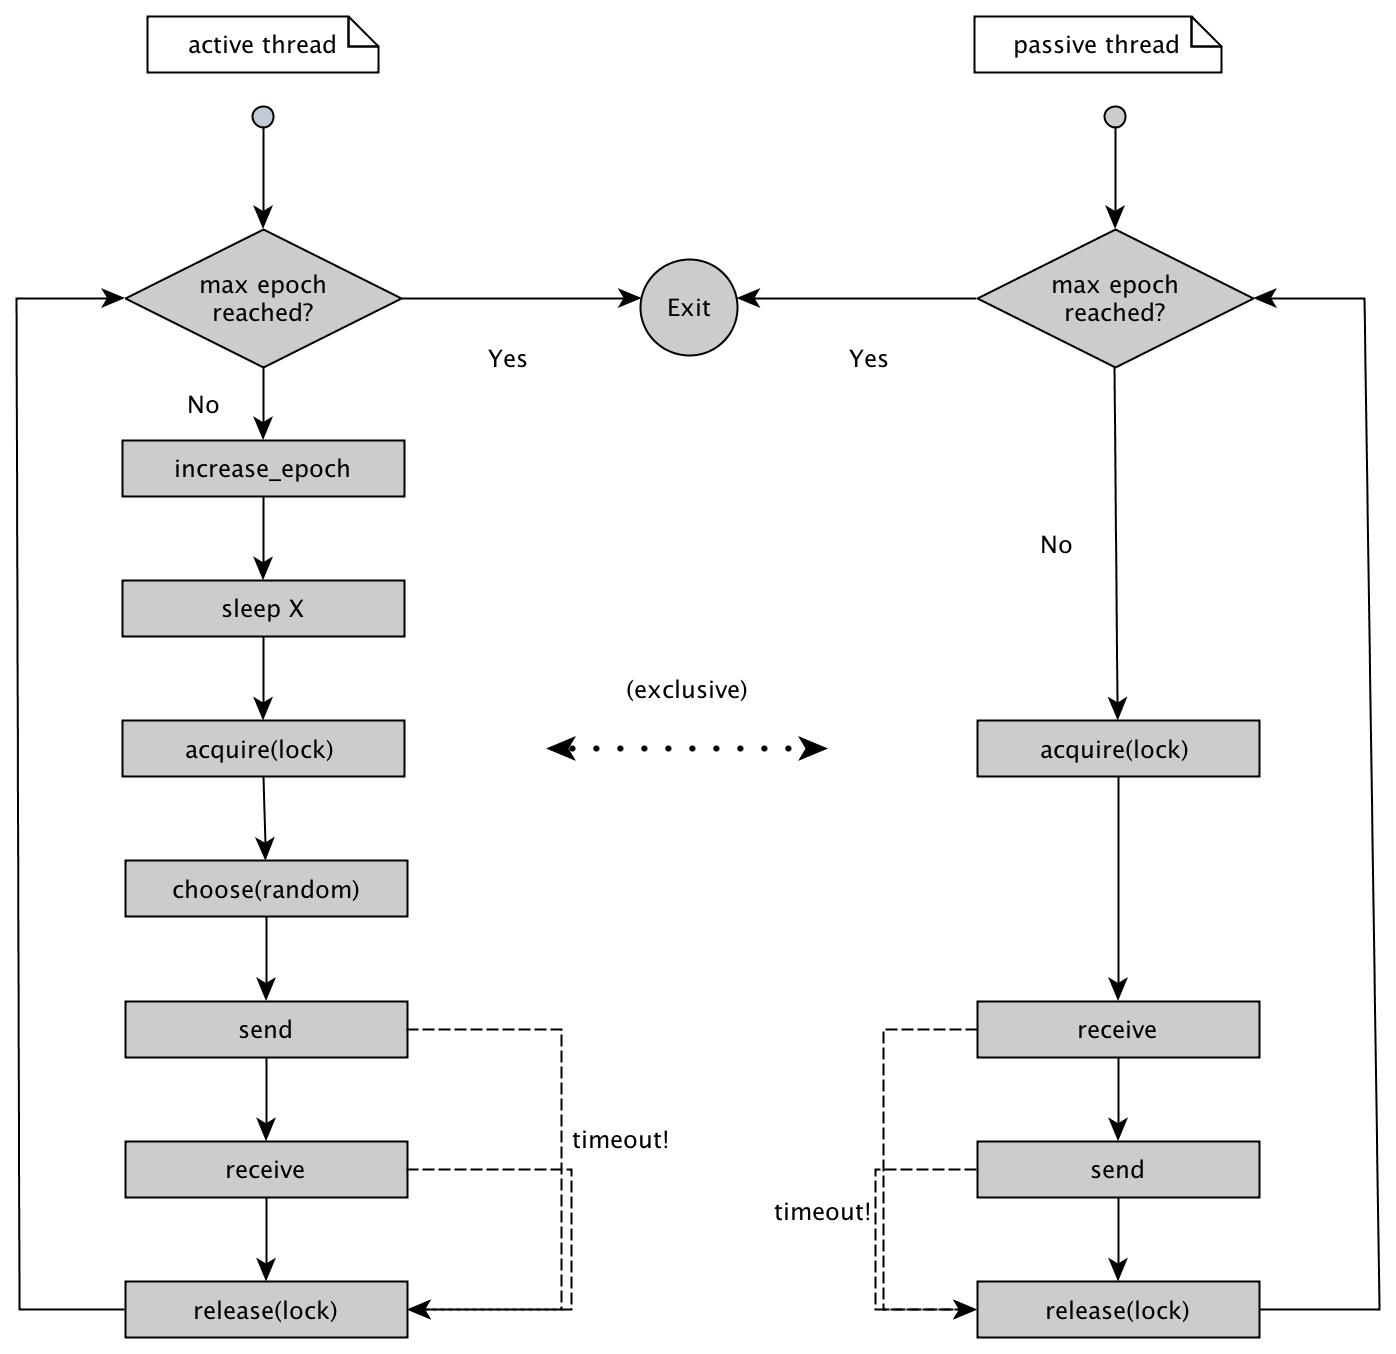
\includegraphics[scale=0.25]{flow_diag.jpg}
    \end{center}
    \caption{Flow diagram of the threads}
    \label{fig:flow_diag}
\end{figure}

Data created this way over one graph is analyzed in R. We compare multiple runs of an experiment over one graph and experiments inbetween graphs. The results are visualized as graphs.

\end{document}
